\documentclass[../../dissertation.tex]{subfiles}
\begin{document}

Defining the search problem in this model is similar to the coined quantum walk
case. The oracle still inverts the sign of a certain state and amplifies it,
and the system's state will still be described by equation
\eqref{eq:sysStateSearch}. However, instead of using a coin, the staggered
model takes advantage of the notions of cliques and tessellations, as was shown
in chapter \ref{sec:chap3StagWalk}, which means the unmodified evolution
operator has to be defined for an undirected complete graph.
\begin{figure}[!h]
	\centering
	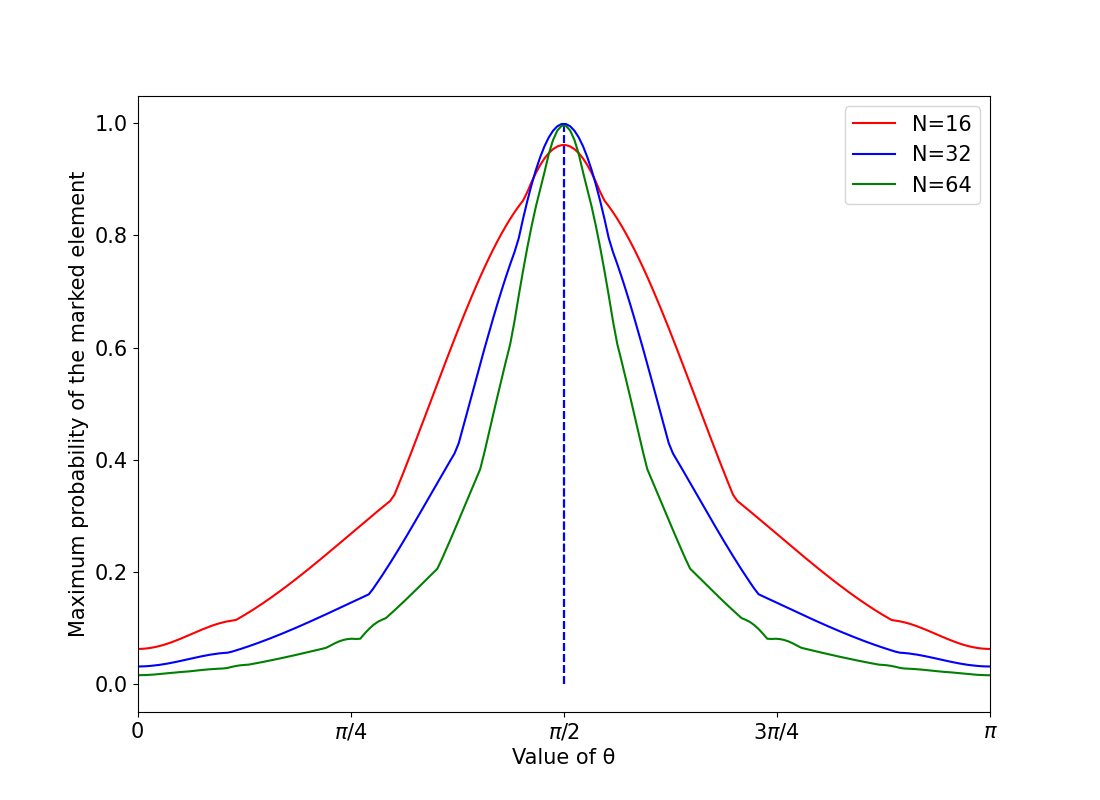
\includegraphics[scale=0.40]{img/StagQuantumWalk/Search/Theta163264.png}
	\caption{Maximum probability of the marked element as a function of the value of $\theta$ plotted from $0$ to $\pi$, for complete graphs of size $N=64$, $128$ and $256$.} 
	\label{fig:stagMultTheta}
\end{figure}\par

As was previously seen, a complete graph is defined as a simple undirected
graph where each pair of distinct vertices is connected by a unique edge.  This
is a special case, because this is the only connected graph that can be covered
by a single tessellation, due to the fact that the graph is it's own clique. The
minimum tessellations required to cover this structures are defined by the one
clique that encompasses all $N$ nodes of the graph
\begin{equation}
	\mathscr{T}_{\alpha} = \{\{0,1,2,...,N-1\}\}.
\end{equation}
The associated polygon can then be described as the balanced superposition of
all the nodes in the graph
\begin{equation}
	\ket{\alpha} = \frac{1}{\sqrt{N}} \sum_{v=0}^{N-1} \ket{v}.
\end{equation}
The Hamiltonian, as defined in equation \eqref{eq:StagHamil}, is 
%TODO: \textcolor{red}{falta índice no somatório}
\begin{equation}
	H_\alpha = 2\sum_0^1\ket{\alpha}\bra{\alpha} - I = 2\ket{\alpha_0}\bra{\alpha_0} - I
\end{equation}\par
The unmodified evolution operator from equation \eqref{eq:stagWalkUnmodOp}
\begin{equation}
	U = e^{i\theta_{k}H_{k}}...e^{i\theta_{2}H_{2}}e^{i\theta_{1}H_{1}}
\end{equation}
reduces to the single Hamiltonian case
\begin{equation}
	U = e^{i\theta H_\alpha}.
	\label{eq:stagQWSearchUnmodEvo1}
\end{equation}
The choice of the value of $\theta$ is quite important, since maximum probability
is achieved at $\theta = \frac{\pi}{2}$, as shown in figure
\ref{fig:stagMultTheta}.
\begin{figure}[!h]
	\centering
	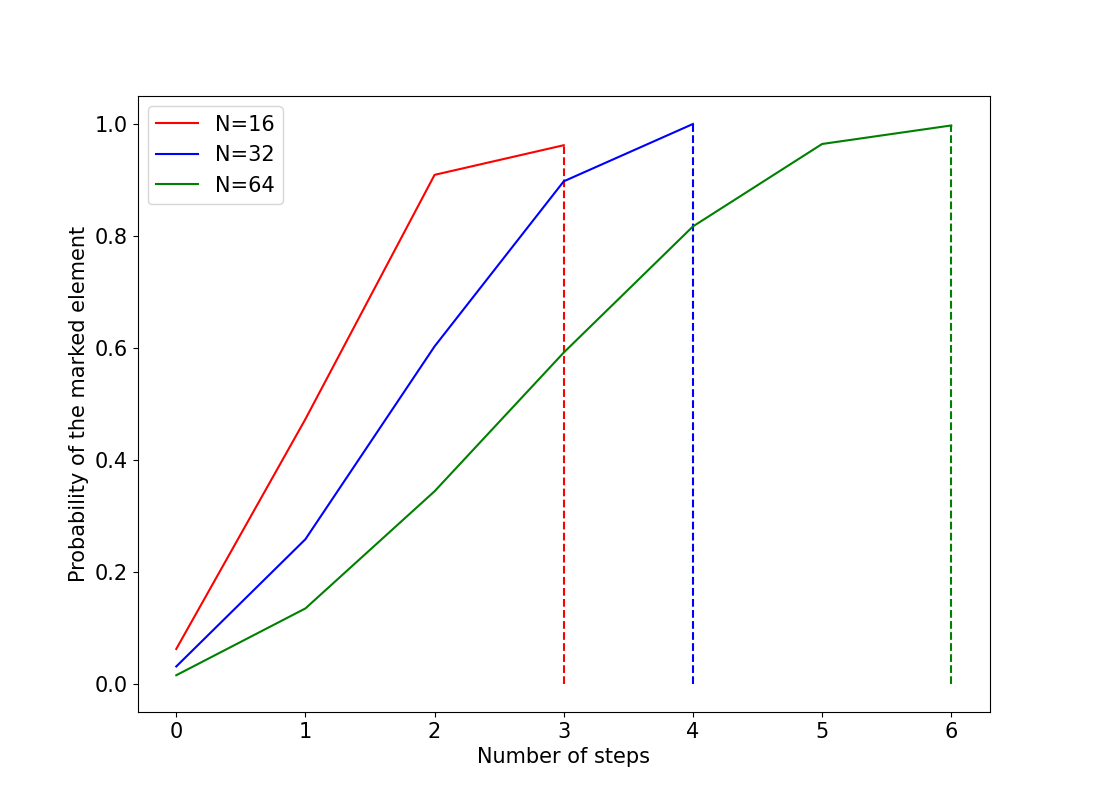
\includegraphics[scale=0.40]{img/StagQuantumWalk/Search/163264.png}
	\caption{Probability of one marked element in the staggered quantum walk search, as a function of the number of steps, for complete graphs of size $N=16$, $32$ and $64$.}
	\label{fig:StagSearch}
\end{figure}\par
Since $H_\alpha^2 = I$, equation \eqref{eq:stagQWSearchUnmodEvo1} can be
rewritten as
\begin{equation}
	U = e^{-i\frac{\pi}{2} H_\alpha} = \cos{\frac{\pi}{2}I} + i\sin{\frac{\pi}{2}H_\alpha} = i H_\alpha = i(2\ket{\alpha_0}\bra{\alpha_0} - I).
\end{equation}\par
Having defined the evolution operator associated to the complete graph,
the next step is to use the oracle
\begin{equation}
	\mathcal{O} = I_N - 2\ket{0}\bra{0},
\end{equation}
to create the modified evolution operator associated with the search
\begin{equation}
	U' = U\mathcal{O}.
	\label{eq:stagSearchSimulModEvoOp}
\end{equation}\par
The walk achieves the same result as Grover's algorithm after
$\frac{\pi}{4}\sqrt{N}$ steps, as shown in figure \ref{fig:StagSearch}. This
plot also shows that the probabilities converge to $1$ as $N$ increases.
Because time is discretized, deviations to the ideal number of steps will
matter less for bigger values of $N$.
Unlike Grover's algorithm, however, the parameter $\theta$ can be changed in
order to alter how many iterations are required to achieve maximum probability
of the marked element. Combined with the fact that one has control over which
structure this search problem is performed, the staggered quantum walk search is
more general than Grover's search, both being equivalent
when a complete graph is considered and $\theta = \frac{\pi}{2}$.\par
Finally, the next section will present the search problem using the
continuous-time quantum walk model. Since time is not discretized, a finer
control over the evolution is possible. This will have significant impact when
translating the algorithm to a quantum circuit, since it will be seen that
circuit depth will not scale with an increase in time. 

\end{document}
